\documentclass[12pt]{article}
\usepackage{helvet}
\renewcommand{\familydefault}{\sfdefault}
\usepackage{hyperref}
\usepackage[english]{babel}
\usepackage[utf8]{inputenc}
\usepackage{amsmath}
\usepackage{graphicx}
\usepackage{cite}
\usepackage{xspace}
\usepackage{algorithmicx}
\usepackage[noend]{algpseudocode}
\usepackage{algorithm}
\usepackage[colorinlistoftodos]{todonotes}
\usepackage{setspace}
\onehalfspacing

%\usepackage[notablist,nofiglist]{endfloat}

% Add Yield as a pseudocode command
\algnewcommand\algorithmicyield{\textbf{yield}}
\algnewcommand\Yield{\algorithmicyield{} }%

% Add Continue as a pseudocode command
\algnewcommand\algorithmiccontinue{\textbf{continue}}
\algnewcommand\Continue{\algorithmiccontinue{} }%

% Add Break as a pseudocode command
\algnewcommand\algorithmicbreak{\textbf{break}}
\algnewcommand\Break{\algorithmicbreak{} }%

% Non-useless comments
\algrenewcomment[1]{\(\triangleright\) #1}%

% Have a command for vocab words
\newcommand{\vocab}[1]{\textbf{#1}\xspace}

\begin{document}

\title{vg: the variation graph toolkit}

\author{Erik Garrison}

\maketitle

\begin{abstract}
Reference genomes provide a prior to guide our interpretation of new sequence data.
However, they have a fundamental limitation in that they only represent one version of each locus, whereas
in a population or species there is in general a distribution of related sequences at each locus.
Mapping new data to a single sequence from this distribution can introduce bias and other problems.
To allow the representation of alternate genomes in our reference system, we develop \emph{variation graphs}, which are bidirectional DNA sequence graphs with embedded paths that describe sequences of interest as walks through the graph.
Here we enable the practical use of variation graphs at human genome scale
by building a toolkit of computational methods for the creation, manipulation, and utilization of these structures.
Our approach generalizes fundamental aspects of resequencing analysis (assembly, alignment, variant calling, and genotyping) to operate on variation graphs.
\end{abstract}

\section{Introduction}

Where genomes are small and sequences from different individuals can be reliably isolated, we can understand variation by assembling whole genomes and then comparing them via whole-genome comparison approaches \cite{mummer}.
In practice, complete genomes are rare, and we require prior information to reduce the cost of our efforts.
The genomes of organisms of interest (such as \emph{Homo sapiens}) are often large \cite{pmid11237011}, and would be costly to work with this way.
Or, they may simply be difficult to completely assemble reliably using cost effective technology (for example, despite extensive efforts and its importance for public health, the current reference for \emph{Plasmodium falciparum} still contains 80 gaps in 250 megabases \cite{pfalciparum, pfalciparumweb}).

We reduce the cost of inference of new genomes by using a suitable prior--- in most cases, a genome of a closely-related individual.
We align sequence reads from the new sample against a single high-quality reference genome.
While expedient, this approach biases our results towards a reference that may poorly represent alleles present in the sample we are attempting to characterize.
We would like to align to a genome that is as similar to our sample as possible, ideally a ``personalized'' reference genome \cite{Yuan_2012}.

We expect to infer new genomes most accurately when they are well-represented by the prior represented by the reference genome.
As a linear reference genome is fundamentally unable to incorporate the genetic information we have available, we are led to ask what structure could include this information.

The natural computational structure for doing so is the sequence graph.
These have a long history of application to problems which require the representation of multiple genomes or ambiguities in the same structure.
For example, multiple sequence alignments have a natural representation as partially ordered sequence graphs \cite{lee2002POA}.
The total information available in a shotgun sequencing data set set can be compressed into a string graph, in which single-copy sequences are represented uniquely and repeated sequences unresolvable due to read lengths are collapsed into single entities \cite{myers2005, simpson2010}.
A similar structure which has good scaling properties when applied to the problem of genome assembly is the de Bruijn graph, which records the relationships between unique $k$-mers of a set of sequences with edges that link pairs of $k$-mers for which the suffix of one $k$-mer is the prefix of the next \cite{iqbal2012}.
The variant call format (VCF) \cite{danecek2011}, which is a common data format for describing populations of genomes, does not explicitly define a graph model, but can be understood as defining a partially ordered graph similar to those used in multiple sequence alignment. 

To serve as a generalized reference system, we propose a general model which allows us to represent these different kinds of sequence graphs. We then implement this model in a practical software environment for operating with them at the multi-gigabase scale: {\tt vg}. Finally, we explore the use of the model for resequencing by constructing whole human genome graphs from a population reference and aligning short read sequencing data against it.

\section{Model}

We define a variation graph to be a graph with embedded paths $G = ( N, E, P )$ comprised of
a set of nodes $N = n_1 \ldots n_M$,
a set of directed edges $E = e_1 \ldots e_L$,
and a set of paths $P = p_1 \ldots p_Q$ which describe transformations from the graph space into a set of sequences.

Each node $n_i$ represents a sequence $seq(n_i)$ which is built from an arbitrary alphabet ${ \cal A }$.
For DNA sequences, we might use ${ \cal A } = \{ {\tt A, T, G, C, N} \}$, but in principle the model can be based in any alphabet.
Nodes may be traversed in either the forward ($+$) or reverse direction ($-$), with the sequence being reverse-complemented in the
$-$ direction.  In general we will use simple variables such as $i$ to indicate a strand of a node (forward or reverse) with $\bar \imath$
for its reverse-complement. By this definition $seq(n_i) = revcomp(seq(\overline{n_i}))$.

Edges represent linkages between nodes that are allowed to be followed in representing longer sequences as paths through the graph.
Edges can be identified with the ordered pairs of node strands that they link, so we can write
$e_{i \rightarrow j} = ( i, j ) $.  In fact this defines one strand of an edge.  Edges also can be traversed in either forward or
reverse direction, with the reverse strand defined by $\overline{e_{i \rightarrow j}} = (  {\bar \jmath}, {\bar \imath} )$.

We define paths as alignments to a walk through the graph.  Explicitly, a path is a series of ``mapping'' operations, each
describing the segment of the path derived from a single node, $p = m_1, \ldots, m_{|p|}$.  Each mapping $m$ can be written
as $( (n, o), e_i \ldots e_{|m|} )$, where $n$ is the node strand, $o$ is the zero-offset start position on the strand ($0 \le o < |n|$),
and each $e_i$ is an ``edit'' which copies or replaces a segment of the node sequence.  In {\tt vg} we encode $e$ as $(f, t, s)$
where $f$ is a length in the node (``from length''), $t$ is a length in the derived sequence (``to length''), and $s$ is an optional
replacement literal sequence of length $t$.  Edges traversed in a path are implicitly defined by the node strands of neighboring mappings.
If all the edits are copies then we say that the path is {\em fully embedded} in the graph.

Figure \ref{fig:minimhc} provides a visual explanation of this model using a small fragment of an assembly of MHC haplotypes.

\begin{figure}[t]
\centering
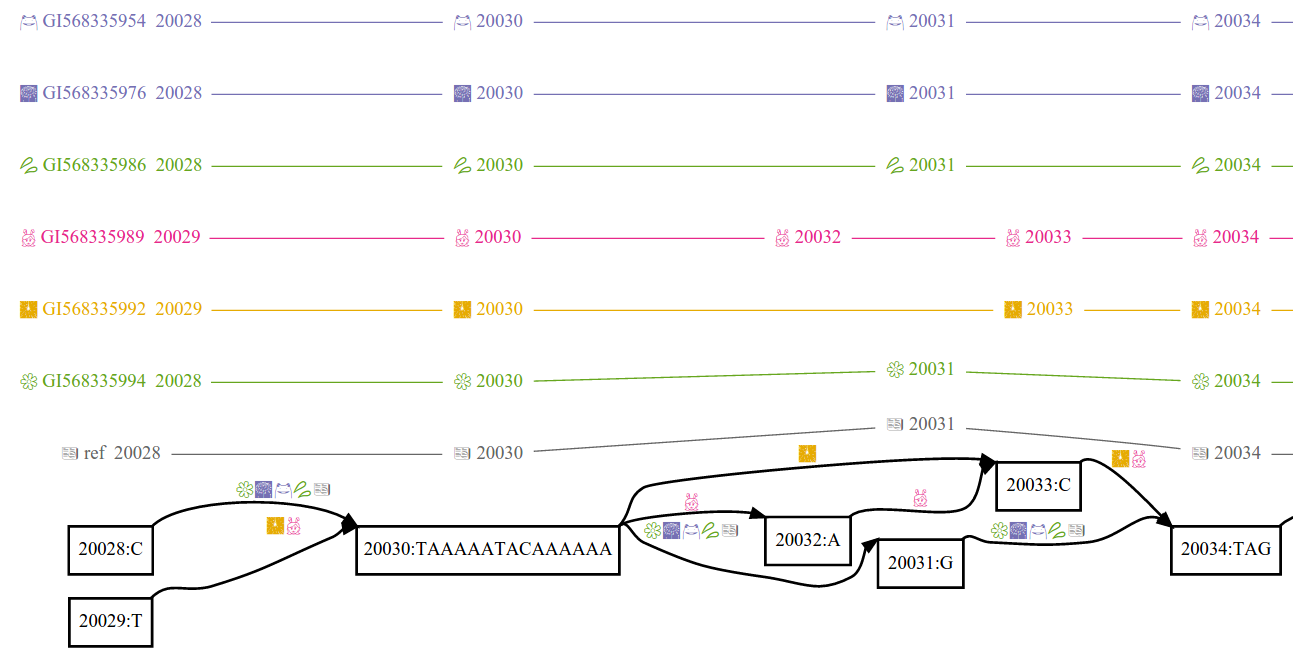
\includegraphics[width=1.0\textwidth]{figures/minimhc}
\caption{\label{fig:minimhc}
  A visualization of a fragment of the MHC variation graph.
  The graph nodes and edges are written at bottom. The edges flow across the tops of the nodes, which indicates in this visualization that they are on the forward strand of the graph and not inverting.
  Paths are described in a matrix above the graph.
  The path name (shown at left) is hashed into a space of 8 colors and 766 Unicode characters (emoji) to provide stable and non-overlapping visual motifs for hundreds of paths.
  These colored pictographs are used to annotate parts of the graph, in this case the edges are labeled with the paths that cross them.
  Visualizations of this type are produced using {\tt vg view -dpn}.
}
\end{figure}

\section{Operations on the graph}

Using two operations we can construct, extend, and modify variation graphs to incorporate new genomes.
\emph{Alignment} provides a description of the optimal set of edits to the graph which would be required to fully embed a given sequence in it.
\emph{Editing} is the process by which we modify the graph to embed the paths describing some set of alignments.

\subsection{Editing}

A fundamental operation on the variation graph is $edit(G, P)$, where the graph $G$ is extended to include the sequences described by paths $P$.

If the nodes of the graph have single-base labels, then they are atomic and need not be split to allow the incorporation of new elements to the graph.
To edit an atomic graph, we only add edges and new nodes representing novel sequence.
We walk the mappings of the alignment through the graph.
We make no changes for matches.
For insertions, substitutions, and soft clipping\footnote{Soft clips are insertions at the end of an alignment.}, we add the novel sequence from the alignment as new nodes in the graph.
For deletions we add edges between existing nodes in the graph.

To edit a non-atomic graph, where the node labels may be of arbitrary length $> 1$, we would first prepare the graph by walking the mappings of any alignments we want to add and cutting the nodes at the positions where we would integrate new sequences.
We record a translation of the node coordinate space to project the alignments mapping positions (which are against the old version of the graph) into the cut graph.
After doing this for any alignments we want to include, we include them by collecting the unique novel subpaths relative to the graph and adding these into the graph at the new cut points.

We implement this editing method as \href{https://github.com/vgteam/vg/blob/fbcb6e62/src/vg.cpp#L4846-L4912}{{\tt VG::edit}}, which consumes a set of paths (possibly from alignments) and extends the graph destructively to fully embed them as paths.

\subsection{Alignment}

An \emph{alignment} is a function that describes a transformation between two sequences.
In our context, one of these sequences is embedded in a graph.
Alignments to the graph look very much like alignments between a pair of linear sequences.
However, we must describe the basis sequence we align against relative to the graph.
We can do this using a \emph{path} through the graph, and describing edits against it.
In {\tt vg}, this non-embedded path is an \emph{alignment}.

We implement efficient local alignment to variation graphs by developing a SIMD-accelerated\footnote{Single input multiple data (SIMD) instructions allow vectorized mathematical operations in a single machine instruction, and can be used to greatly speed up algorithms which may be implemented in terms of operations on vectors.} string to graph alignment algorithm. We then enable alignment against completely generic graphs by a transformation process that projects a cyclic and bidirectional graph into an acyclic, unidirectional (single-stranded) graph which preserves the sequence space of the original graph up to a given length.

\subsubsection{Background}

Alignments between strings and graphs have been used in several contexts in bioinformatics.
We draw on this work to implement a local alignment method for generic variation graphs.

The canonical approach for aligning acyclic sequence graphs is partial order alignment (POA) \cite{lee2002POA}.
In POA, we can align partially ordered graphs (DAGs) to each other using a basic generalization of the traditional dynamic-programming based alignment algorithms for pairs of sequences.
POA generalizes the scoring recurrence such that we consider all possible inbound positions in the graph when deriving the score for a new node.
This model requires that the graph be acyclic, as we cannot derive the score for a new node until we have determined it for all of our predecessors.
\footnote{An implementation of \href{https://sourceforge.net/projects/poamsa/}{POA-msa} has been available since 2002. It has been used for multiple sequence alignment and more recently recently for \href{https://simpsonlab.github.io/2015/03/30/optimizing-hmm/}{correcting nanopore sequencing errors}.}

Assembly algorithms that construct a deBruijn graph do so by aligning new sequences into a deBruijn graph, and then editing the graph to include them by adding the kmers of the new sequence \cite{iqbal2013, zerbino2008}.
Recent work utilizes this same concept to implement an aligner for mapping short reads into population reference graphs \cite{prg2015}, which is very similar in spirit to our work but does not generalize to arbitrary sequence graphs.

The general case of alignment between cyclic graphs was described by \cite{myers1989} in the context of the alignment of regular expressions.
As our sequence graphs are models of regular languages, they can be considered equivalent to regular expressions, so we understand this result to hold for variation graphs as well.
By transforming our graph from a cyclic to acyclic format, we produce a performant implementation of the limited case of alignment between strings and regular languages. However, we have not implemented the general case of alignment between regular languages, and know of no available software methods that implement it.

\subsubsection{SIMD-accelerated local alignment}

We implement a SIMD-accelerated version of partial order alignment, which we term ``graph striped Smith-Waterman'' \href{https://github.com/ekg/gssw}{GSSW}.
This method extends an implementation \cite{zhao2013} of Farrar's the striped Smith Waterman (SSW) algorithm \cite{farrar2007} to operate over graphs and retain its scoring matrices for later traceback.
GSSW generalizes all aspects of SSW to operate over sequence DAGs, including affine gap penalties, and is around 6 times faster than a non-SIMD based implementation of POA.

We interface with GSSW by \href{https://github.com/vgteam/vg/blob/fbcb6e62/src/vg.cpp#L6461-L6532}{transforming our graph into the internal graph used by GSSW}.
This graph is acyclic and only represents a single strand of the DNA.
In order to align against completely general, bidirectional sequence graphs (such as those with cycles and inversions), we can apply several transformations to the graph first to generate a DAG with the property that we can find any sequence up to a given length from our source graph in it.

These two operations are $unfold$, which expands the graph to include its reverse complement where accessible via an inversion, and $kDAGify$, which unrolls strongly connected components of the graph ``far enough'' that we are guaranteed to be able to find any sequence of length $k$ in the source graph in the unrolled one.
This allows us to align any sequence of up to length $k$ against a completely general variation graph.
Through these steps we retain a mapping from old node ids to new ones, which we will use to project alignments to the transformed graph back into our base coordinate space.

\subsubsection{Unfolding}

In \href{https://github.com/vgteam/vg/blob/fbcb6e62/src/vg.cpp#L8289-L8400}{{\tt VG::unfold}} we use a breadth first search starting at every inverting edge in the graph to explore the reverse complemented portions of the graph that we reach in some length $k$ from the inverting edge.
We then copy this subgraph, take its reverse complement, and replace the inverting edges connecting it to the forward strand of the graph with non-inverting ones.
If $k$ is greater than any length in our graph, then we will duplicate the entire reverse complement of the graph on the forward strand, effectively doubling the size of the graph if we have any inversions in it, as shown in figure \ref{fig:unfold}.

\begin{figure}[t]
\centering
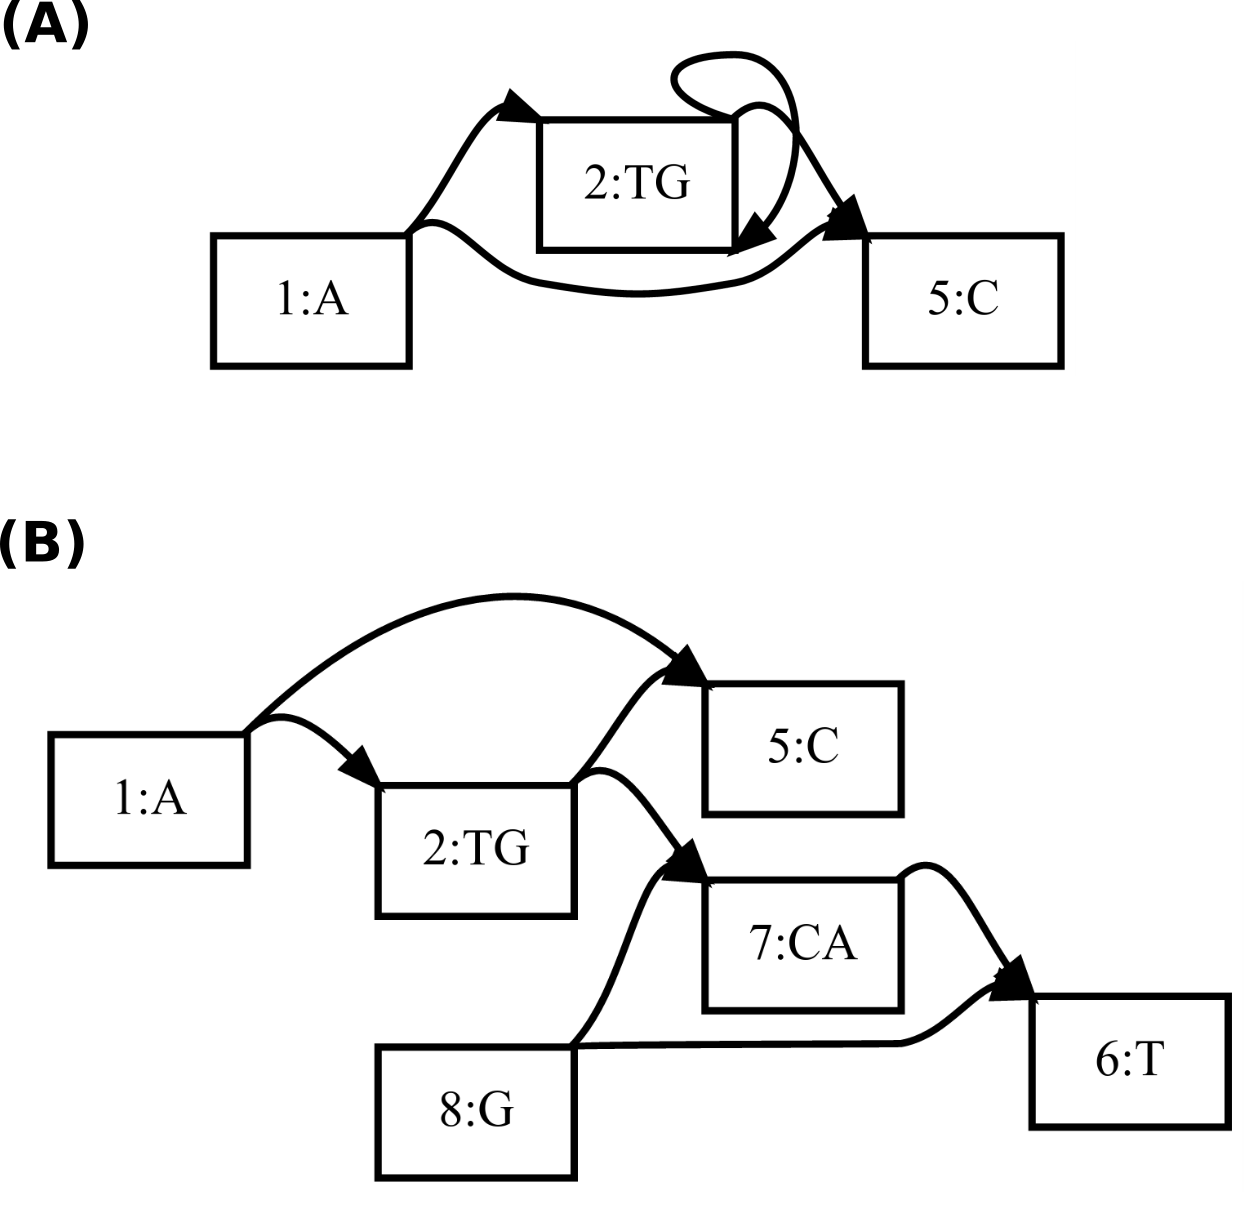
\includegraphics[width=1.0\textwidth]{figures/unfold}
\caption{\label{fig:unfold}
  The starting graph (A) has an inverting edge leading from the forward to reverse strand of node 2.
  In (B) we unroll the graph with $k$ greater than the length of the graph, which materializes the implied reverse strand as sequence on the forward strand of new nodes.
}
\end{figure}

\subsubsection{kDAG-ification}

Variation graphs may have cycles.
These are useful as compact representations of copy number variable regions, and arise naturally in the process of genome assembly.
However, partial order alignment cannot handle these structures, and so we must convert them into an approximately equivalent acyclic graph in order to align with GSSW.
To do so, we unroll cyclic structures by copying their internal nodes an appropriate number of times to allow a given query length to align through the unrolled version of the component.

We first detect all strongly connected components by using a \href{https://github.com/vgteam/vg/blob/fbcb6e62/src/vg.cpp#L3508-L3552}{recursion-free implementation} of Tarjan's strongly connected components algorithm \cite{tarjan1972depth}.
Then, we copy each strongly connected component and its internal edges into a new graph.
We greedily break edges in this graph that introduce cycles.
Now, we k-DAGify the component progressively copying the base component and for each edge between nodes in the component, connecting from the source node in the previous copy to the target node in the current copy.

We use dynamic programming to track the minimum distance back through the graph to a root node outside the component at each step.
When this reaches our target $k$, we stop unrolling, and add the expanded component back into the graph by reconnecting it with its original neighborhood.
For each copy of a node in the DAG-ified component we copy all of its inbound and outbound edges where the other end of the edge lies outside the strongly connected component.
The resulting graph is acyclic and supports queries up to length $k$ on the original graph provided the translation between the new graph and the source one.
Figure \ref{fig:kdagify} provides a visual description of the process.

\begin{figure}[t]
\centering
\includegraphics[width=1.0\textwidth]{figures/kdagify}
\caption{\label{fig:kdagify}
  The starting graph (A) and a representation without sequences or sides to clarify the underlying structure (B).
  In (C) we have unrolled one step ($k = 2$). In (D), $k = 4$, (E) $k = 10$, and (F) $k = 25$.
}
\end{figure}

\subsection{Construction}

We can build a trivial graph without any bifurcations and a single acyclic component from any linear reference sequence.
A more interesting graph may be generated by a series of align, edit operations.
Assemblies of this type may be generated by a variety of methods, and we implement interfaces to read in the most common forms.

\subsubsection{From population-scale sequencing results}

A VCF file encodes a sequence DAG.
We can interpret it as a multiple sequence alignment of individual genomes and a single reference.
As such, it is straightforward to build a variation graph from population variation data in a VCF file.
We do this using the same technique as in {\tt VG::edit}.
First, we convert the alleles in the VCF file into mappings to a graph made of only the reference sequence. 
We then edit this graph using the mappings, incorporating the sequences given by the alleles in the VCF record into the graph. 

In standard practice, we ignore the haplotype information in the VCF file and build the graph so as to allow all possible recombinations between successive variant loci.
This haplotype-agnostic approach has advantages of simplicity and ubiquity.
Even data providers with closed access policies will release information about the variants discovered in their cohorts, which provides a valuable resource when examining new individuals even if we do not have the complete haplotype information of the source genomes \cite{exac2015}.
However, there are valuable uses for the haplotypes, and storing this haplotype information efficiently is an area of active work among other collaborators on {\tt vg} are exploring generalizations of the positional Burrows Wheeler Transform (PBWT) \cite{durbin2014}.\footnote{Adam Novak, a collaborator on the {\tt vg} project, has implemented a generalization of the PBWT to graphs in xg. This generalization (gPBWT) is designed for efficient haplotype matching and frequency queries, but does not provide efficient positional queries.}

\subsubsection{\emph{De novo} assemblers}

Many \emph{de novo} assembly algorithms utilize a graph model internally to represent ambiguity in the sequencing data they are applied to.
They assemble a graph by overlapping reads or their $k$-mers, then generate contigs as regions of this graph with low diversity in the input sequencing data.
Provided a \emph{de novo} assembler implements a compatible data model to the variation graph, we can build variation graphs from intermediate representations.
In {\tt vg} we support the \href{https://github.com/pmelsted/GFA-spec}{graphical fragment assembly (GFA) format}, which is a community standard serialization for bidirectional sequence graphs.
In theory this allows interchange of graph data between different assemblers and sequence graph algorithms, but in practice the format is young and tools have not coalesced around a completely stable schema.

\subsubsection{Progressive variation graph assembly}

Provided the {\tt VG::align} and {\tt VG::edit} functions, we can generate progressive assemblies in much the same manner as is done in POA.
We align each sequence and edit the graph to include it in turn.
The resulting graph contains all input sequences as embedded paths.
We implement this technique as the \href{https://github.com/vgteam/vg/blob/fbcb6e62/src/main.cpp#L674-L1248}{multiple sequence/graph aligner {\tt vg msga}}, and have applied it to assemble long sequences from the human MHC as described in section \ref{sec:MHC}.

\section{Indexing variation graphs}

It is practical to disable editing of the graph when we want to use the graph as a reference system.
In doing so, we have an opportunity to derive a more compact representation for the graph that is static but allows efficient queries of the graph.
Such representations are termed ``succinct'' when they occupy only a small constant factor more space than that required to store a compressed version of their source data.
In {\tt vg} we use two indexes based on succinct data structures to enable the alignment of sequences to large graphs using low memory: a succinct variation graph index ({\tt xg}), and the generalized compressed suffix array ({\tt GCSA2}).

\subsection{Succinct graph representation ({\tt xg})}

Our core implementation of variation graphs, \href{https://github.com/vgteam/vg/blob/fbcb6e62/src/vg.hpp#L196-L1146}{{\tt vg::VG}}, is optimized for efficient runtime for editing and transformation operations.
These needs mean we must store a dynamic version of the graph, which we do using unordered maps that are optimized for runtime and not memory overhead.
We have estimated that more than 300G of RAM would be necessary to load the entire graph into main memory.
Furthermore, serialization overheads mean that loading this graph would take up to an hour.
Editing operations are mostly local, and so this poses little problem for many use.
However, it prevents us from working with the entire graph in one context.

When using a variation graph as a reference system, we are unlikely to need to modify it.
As such we can compress it into a system that provides efficient access to important aspects of the graph.
Specifically, we care about the node and edge structure of the graph and queries that allow us to extract and seek to positions in embedded paths.
We would like to be able to query a part of the graph corresponding to a particular region of a chromosome in a reference path embedded in the graph.
Similarly, if we find an exact match on the graph using {\tt GCSA2}, we would like to load that region of the graph into memory for efficient local alignment.

We implement a succinct representation of the graph in the \href{https://github.com/vgteam/xg}{{\tt xg}} library.
We do so using data structures from \href{https://github.com/simongog/sdsl-lite}{SDSL-lite}, which provides \href{https://en.wikipedia.org/wiki/Succinct_data_structure#Succinct_dictionaries}{rank/select dictionaries} that we use to navigate compressed vectors that record the labels and id space of the nodes, edges, and paths of the graph \cite{okanohara2007}.
Our model is summarized visually in figure \ref{fig:xg}.

\subsubsection{Storing the nodes of the graph}

We first concatenate node labels to generate the node sequence vector $V_s = seq(n_1) + seq(n_2) + \ldots + seq(n_{|N|})$.
We store this as a compressed integer vector using the minimum required number of bits per base (which is typically 3 bits, as we need to represent ${\tt A, T, G, C, N} \}$).
In a second bit vector $V_b : |V_b| = |V_s|$ (the node bit vector), we write 1 at the position corresponding to the first base in every node in $V_s$, and write a 0 for all internal bases.
We then store the node ids in the wavelet tree $V_i$ \cite{grossi2003high}, ordered by their appearance in $V_s$.

By building a rank/select dictionary from $V_b$, we can map from positions in the sequence vector to node ids, and from node ids to ranges in the sequence vector.
For example, we can look up the sequence of a particular node by its id in several steps.
We first query the node id wavelet tree to obtain the rank $n$ of a particular node by its id $i$: $n = rank_{i}(V_i, 1)$.
Then, $select_1(V_b, n)$ will return the position of the start of the $n$th node in the node sequence vector.
In reverse, we can use $rank_1(V_s, n)$ to map from positions in $V_s$ to node ranks, and then find the node id as $V_i[n]$.
Recording the node identifiers in $V_i$ allows us to work with non-contiguous node id spaces, but internally within {\tt xg}, we identify nodes by their rank in $V_s$ and $V_i$.

\subsubsection{A succinct bidirectional encoding of the edges of the graph}

Variation graphs which we are likely to use as a reference system tend to have few nodes with a high in or out degree.
We rely on this tendency to generate a bidirectional index of edges that is optimized for sparsely-connected graphs.

We store the edges of graph, $E$, using a pair of compressed integer vectors $F_e$ and $T_e$.
In each vector, we record information about the edges of each node in a single range of the vector.
We record the ranges of these vectors corresponding to particular nodes by marking bit vectors $F_b$ and $T_b$.

We record the edges in the forward direction in $F_e$.
For each $n_i \in N$ we write its own id into $F_e$.
Then for each edge from that node ($\forall j : e_{n_i \rightarrow j}$) we record the id of the node it goes to ($j$) in a block after the entry for $n_i$.
We record the position of the node blocks in $F_e$ in $F_b$ by marking the node entry with a 1, and leaving edge entries as 0.

$T_e$ and $T_b$ follow the same pattern, but instead of recording the edges from a node, we record the edges to it.
This bidirectional structure allows for fast traversal of the graph.
Note that $|F_e| = |T_e| = |N| + |E|$.
In other words, these vectors encode one entry for each node and edge in the graph.
We can exploit this property to provide a unique rank-based identifier for every node and edge in the entity space of the graph, which is useful for marking subgraphs with particular properties.

We use such a pattern to record the which node strand each edge starts and ends on.
Four additional bit vectors mark whether an edge starts or ends on the forward or reverse strand: $|I_f| = |I_t| = |J_f| = |J_t| = |N| + |E|$.
We first mark all positions corresponding to the node block starts in $F_e$ as 0.
This padding ensures that we are working in the graph's entity space as described by $F_e$.
In $I_f$ we record if an edge in $F_e$ begins on the reverse strand (1) or not (0), and in $J_f$ we do the some for edges as described in $T_e$.
In $I_t$ we store if an edge in $F_e$ goes to the reverse strand (1) or not (0), while $J_t$ lets us do the some for edges as ordered in $T_e$.
In directed graphs these are typically sparse and easily compressible, but they are necessary to represent completely generic graphs.

\subsubsection{Compact path storage allowing positional queries}

In {\tt xg} we develop a compact representation of embedded paths that allows them to be used for $O(1)$ time positional queries.
For each path $p_j$ we store a bit vector $C_p^j$ with the same length as our forward edge vector $F_e$.
We mark 1 in this vector for each element in the graph which occurs in the path at its corresponding position in $F_e$, and a 0 otherwise.

We record the positions of the mappings ($m_1, \ldots, m_{|p_j|}$) of $p_j$ in an integer vector $M_p^j$, where we record the node ranks of the nodes the path traverses in $V_s$.
The strand of each mapping $m$ is marked in a bit vector $S_p^j$ of the same length as $M_p^j$.
We mark 0 if the mapping traverses the node's forward strand and 1 if it traverses the reverse.

Finally, we build a positional index of the path that allows us to determine what node strand of the path is at a given position.
We cache the start position of each node relative to the beginning of the path in $L_p^j : |L_p^j| = |M_p^j|$.
The bit vector $B_p^j$ has the same length as the sequence represented by the path.
For each position in the path where we begin a node, we mark a 1, and leave 0 otherwise.
We can now determine the node at a given position $x$ in the path as $M_p^j[rank_1(B_p^j, x)]$.
Furthermore, we can efficiently determine where in a particular path a node is using the $L_p^j$ vector.
This representation is not lightweight, and does not allow the storage of many paths because it requires $O(\sum_{\forall p \in P}{|p|})$ space.
However, it is an essential component of the index if we wish to query the graph based on the coordinate system of an existing linear reference sequence.

\begin{figure}[t]
\centering
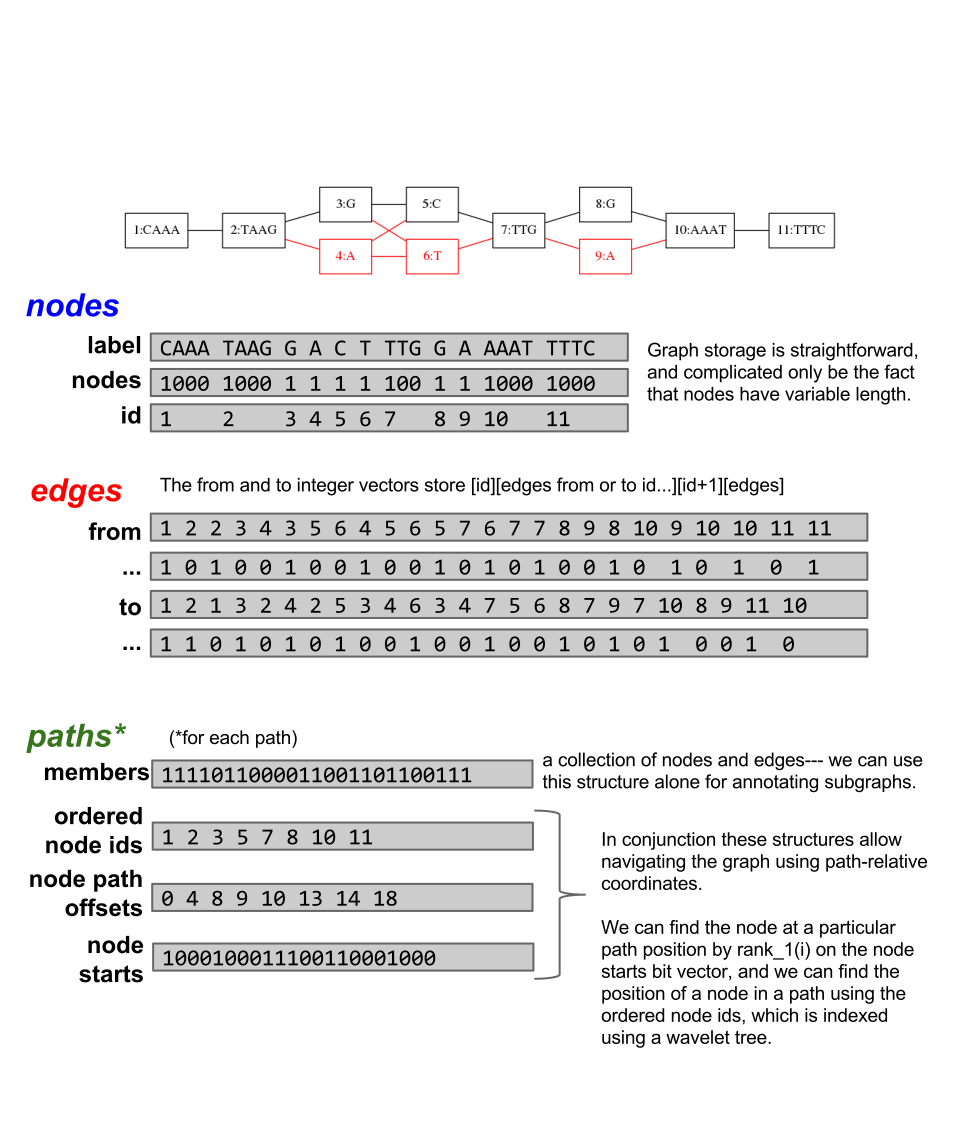
\includegraphics[width=1.0\textwidth]{figures/xg}
\caption{\label{fig:xg}
  A sketch of important components of the {\tt xg} graph index.
  The source graph is at the top of the figure.
  A single path is defined by the nodes and edges in black.
  For simplicity we omit the edge type vectors and the traversal orientation vector as in this directed acyclic graph they would be marked as 0.
}
\end{figure}


\subsection{Sequence queries ({\tt GCSA2})}

Efficient alignment of sequences against large graphs using only dynamic programming is not feasible as it requires $O(NM)$ operations to derive an optimal alignment of a pair of sequences of length $N$ and $M$.
We can substantially improve these bounds by focusing the expensive dynamic programming alignment only in regions of the graph where we find exact matches between the query and our reference.
For linear sequences, the FM-index \cite{fmindex2000, fmindex2005} provides the required functionality to do so.
Based on the Burrows-Wheeler transform (BWT) of a source text \cite{burrowswheeler1994}, the FM-index adds operations that allow the traversal of the suffix array embedded in the BWT.
An auxiliary data structure provides the mapping from BWT positions to positions in the source sequence.
As we can look up exact matches of length $N$ in a suffix array in $O(N)$ operations, the FM-index and other compressed suffix array variants allow us to efficiently localize reads to regions of the reference before applying expensive local alignment algorithms.

Several generalizations of the FM-index to sequence graphs have been developed in recent years.
The generalized compressed suffix array (GCSA) allows sequence queries in populations of genomes represented in a single multiple sequence alignment, but is limited to directed acyclic representations of these collections and requires heuristic optimization to build whole genome indexes \cite{siren2011indexing, siren2014indexing}.
The hierarchical graph FM index (HGFM) implemented in \href{https://github.com/infphilo/hisat2}{HISAT2} allows direct mapping of RNA sequencing reads against a transcriptome model including small sequence variants such as SNPs and indels \cite{kim2015hisat}.
In the HGFM, a global GFM represents the general population, while tens of thousands of local GFMs represent denser variation on a small scale.
Similarly to GCSA, HGFM requires the input graph be acyclic.

Recently, Sirén\footnote{Jouni Sirén is currently a postdoctoral fellow in computational genomics at the Sanger.} has developed \href{https://github.com/jltsiren/gcsa2}{GCSA2}, which generalizes the GCSA/GFM model to use positionally-labeled deBruijn graphs as input.
We implement global alignment in {\tt vg} by transforming the variation graph into a deBruijn graph with positional labels that indicate where in the source graph a particular kmer starts and ends.
{\tt GCSA2} can then generate a GCSA from this labeled deBruijn graph, which we utilize during queries of the sequence space of the graph.

MEMs are matches between a query and a reference system that cannot be extended in either direction along the query while still matching some sequence in the reference system.
Super-maximal exact matches (SMEMs) are MEMs that are not contained by any other MEM.
As in {\tt bwa mem} \cite{li2013bwamem}, we use SMEMs to seed local alignment of reads.
{\tt GCSA2} provides a nearly-complete generalization of the FM-index to sequence graphs.
As it provides functions to traverse the suffix tree embedded in the GCSA, we can use it to derive maximal exact matches (MEMs) against the source graph in a single pass over our query.

\section{Resequencing against the graph}

Provided compact representations of the graph and the sequences of paths through it, we are able to support resequencing experiments where a graph is used as the reference system.
Here we describe the two essential phases of this process: the global alignment of reads to a large graph, and the detection of novel variation against the graph.

\subsection{Global alignment}

We begin global alignment by deriving the MEMs for a query relative to our reference system.
MEMs that are high-abundance may be filtered out by counting the number of occurrences in the graph using \href{https://github.com/jltsiren/gcsa2/releases/tag/v0.6}{{\tt GCSA2}'s $count$ function}, which uses techniques from document counting in compressed indexes to generalize the range counting that is possible in a compressed suffix array to GCSA.
This allows us to avoid MEMs that have hundreds of thousands of hits in our index without extracting the specific hits from {\tt GCSA2}.

We then cluster these MEMs by exploiting an approximate distance metric on the graph.
If our node id space is locally ordered, then nodes with nearby ids are likely to lie close together in the graph.
We set a parameter to limit the distance at which we cluster, which is usually small (in the range of 5-10 when we have built our graph with a maximum node size of 32).

Now, for each cluster we extract the subgraph of the cluster and a small neighborhood around it from {\tt xg}, and locally align against it using unfolding, kDAGification, and GSSW alignment.
We sort the hits by their GSSW alignment score, and return either the top hit or all hits if multi-mapping results are desired.

Paired end reads may be handled using the approximate locality metric based on node ids.
Where one but not both fragments of a read pair map, we attempt to rescue the failed mate by aligning it in a window around the successful mapping.

For very long reads, where the local dynamic programming can become prohibitively expensive, we break the reads into ``bands'' of a fixed width $w$ with overlap between successive bands of $w/2$.
We then align these bands independently, trim the overlaps from the alignments, and concatenate the results.
This allows {\tt vg} to map reads of arbitrary length, and is used as a core component in the long read progressive assembler {\tt vg msga}.

\subsection{Variant calling}

Variant calling on the graph is similar to variant calling on a linear reference \cite{samtools, garrison2012haplotype}.
To call new variation, we extend the graph with the putative novel alleles from alignments (via $edit$), label the graph with the amount of read support we have, and filter out the portions of the graph with little or no support from the reads.
The resulting graph is a sample-specific graph, and conveys similar information as a \href{http://samtools.github.io/hts-specs/VCFv4.2.pdf}{gVCF} file, which describes both the novel and reference-matching portions of the genome of a particular sample.
Currently variant calling in {\tt vg} is rudimentary and based around a multi-stage ``pileup'', $edit$, and calling pipeline.\footnote{UCSC researchers Glenn Hickey, Adam Novak, Benedict Paten, and Maciej Smuga-Otto have contributed to this effort as part of the Global Alliance for Genomics and Health evaluation of graph reference genomes.}

\section{Results}

We have implemented {\tt vg} in C++11 under an open, distributed software development model.
The \href{https://github.com/vgteam/vg}{{\tt vg} source repository} totals 28k lines of {\tt vg}-specific code, which is augmented by a variety of dependencies (including {\tt xg} and {\tt GCSA2}).

Here we briefly describe several results demonstrating the functionality of {\tt vg}.
All experiments were carried out on the Sanger farm on a dedicated compute node with 256 gigabytes of RAM and 32 2.4GHz AMD Opteron 6378 processors.

\subsection{Software development and continuous integration testing}

All features of {\tt vg} are validated after every update to the source repository using \href{https://travis-ci.org/vgteam/vg}{continuous integration software validation approaches}.
As such, basic tests demonstrate the desired functionality for each feature, in some cases in using a programmatic proof.
For example, we use kmer matching to verify that the kmer space of a graph is equivalent before and after unrolling and kDAGification.
As of this writing, we have implemented 228 tests validating the functionality of the system.

\subsection{The 1000 Genomes Project graph}

The final phase of the 1000 Genomes Project has produced a data set describing the genomes of 2500 humans \cite{1000g2015}.
We transformed the sequence DAG described by the project's released VCF and the GRCh37 reference into a variation graph in 15.5 hours using 32 threads.\footnote{VCF-based construction is parallelized by breaking the build into smaller pieces at particular parts of the reference and concatenating the resulting graphs.}
The resulting graph is 4.5G when serialized to disk, and contains 3.181 gigabases of sequence, which is exactly equivalent to the length of the input reference plus the length of the novel alleles in the VCF file.

\subsection{Indexing the 1000GP graph}

We indexed the 1000GP+GRCh37 graph in two phases.
First, we built the {\tt xg} index using a single-threaded process in 1.5 hours.
This process requires a high amount of RAM as it must load the entire graph into memory. For this bootstrapping process we use a reduced representation of the variation graph that requires 170G of RAM at peak.
The resulting {\tt xg} index is 30G on disk and when loaded into RAM for use by {\tt vg}.

The 1000GP+GRCh37 graph includes some regions that are highly degenerate, where many variants occur in small window.
As our current construction process does not take into account the haplotypes in the VCF file, we include all recombinations between these alleles in our graph, generating small regions of high complexity.
To build the {\tt GCSA2} index, we must remove these regions. Otherwise, the intermediate deBruijn graph will be too large to process in reasonable time.
Using algorithms in {\tt vg mod}, we pruned edges from the graph which induce more than 4 bifurcations in 16bp, and removed any extremely short subgraphs that result from this destructive masking operation.
This transformation preserves the id space of the graph, allowing us to use it as the basis for seed generation against the un-pruned graph.

Then, we transform this pruned 1000GP+GRCh37 graph into an order 16 deBruijn graph.
We were able to distribute the pruning and deBruijn graph generation steps by chromosome across the cluster, so precise timing of this step was not possible, but we estimate it to be in the range of 24 hours on a single 32-core system.
We then built the {\tt GCSA2} index with two steps of prefix doubling, wherein the its construction algorithm uses the positional information in the input deBruijn graph to double the order of the graph (prefix doubling takes us from a graph where $k = 16$ to $k = 32$, and finally $k = 64$).
The {\tt GCSA2} indexing process required 100G of RAM at peak, but minimizes memory usage by implementing most operations using streaming disk-backed sorts.
As such, it required several terabytes of I/O during indexing.
The final step of {\tt GCSA2} indexing required 32.9 hours of wall clock time and 105.3 hours of CPU time.

\subsection{Mapping reads from NA12878}

As a basic test of the functionality of the current implementation of the indexes, we aligned a million reads from an Illumina X10 read set of NA12878 against the graph.
This requires 60 seconds to load the indexes, 67G of RAM, and approximately 145 seconds to align the reads.\footnote{Completed on {\tt vg-fbcb6e62} using paired end mapping and parameters -GX 0.9 -m 10 -c 5}
The mapping rate is 99.4\% = $1 - (6418 / 1e6)$.
Based on this test, we estimate that we are able to align 7000 reads per second on the 32-core machine.\footnote{This will need to be improved by as much as a factor of two to ensure that the method can be used in production on resources available at the Sanger.}
We were not able to complete a whole genome analysis using {\tt vg}'s MEM mapping algorithm in time for this report.

\subsection{An overlap assembly of the MHC}
\label{sec:MHC}

In many contexts we have finished genomes, but not an assembly graph or VCF file suitable for direct transformation into a variation graph. 
To support the use of {\tt vg} in these contexts,
we developed a long read assembler \href{https://github.com/vgteam/vg/wiki/Long-read-assemblies-using-vg-msga}{\tt vg msga}.
This method takes a starting sequence or graph and progressively aligns new sequences to the graph, editing the graph to embed each new sequence as a path until all sequences have been included.
The process is deterministic and complete in that each new sequence will generate an alignment.
New sequences which do not map become new disjoint subgraphs, while homologs will be compressed against each other in the resulting graph.

We applied this method to the GRCh38 alternate alleles for the entire MHC.
Each sequence is between 4.6 and 5 megabases.
We begin with the base reference sequence and add GI568335879, GI568335954, GI568335976, GI568335986, GI568335989, GI568335992, GI568335994, and GI568335997 in turn.
The process requires around on hour on our test machine, producing a graph that serializes to 18M on disk.
We observe that the similarity of the sequences results in a more compact graph than would be expected by concatenating the sequences.
The total sequence length of the input is $38.16 \times 10^6$ bases, whereas the resulting graph contains $10.8 \times 10^6$, a reduction of 3.5 fold.
Figure \ref{fig:DRB1-3123} shows a rendering of a graph generated by {\tt vg msga} using the sequences of one of the MHC genes (DRB1-3123).

% actual counts: 38160773bp, 10802468bp

\begin{figure}[t]
\centering
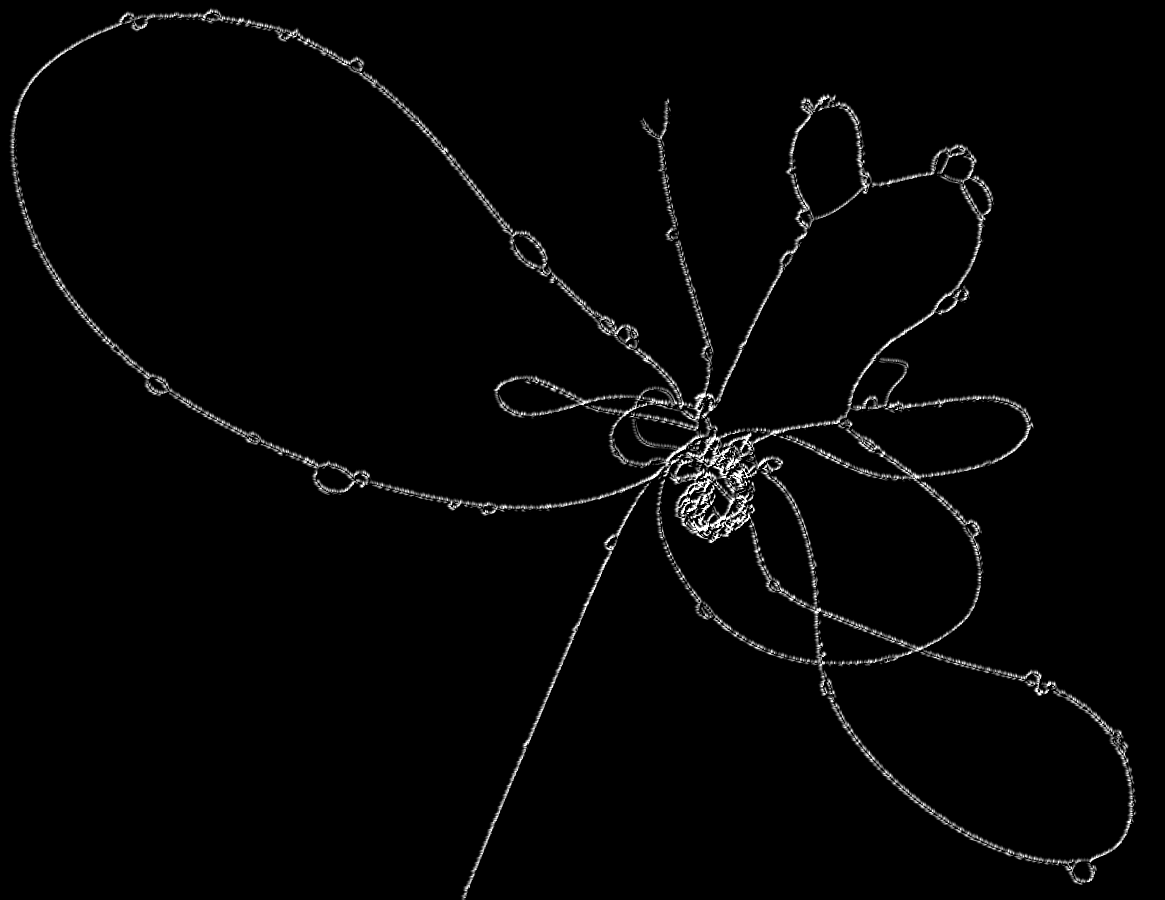
\includegraphics[width=1.0\textwidth]{figures/DRB1-3123}
\caption{\label{fig:DRB1-3123}
  A rendering of a portion of the MHC graph assembled by {\tt vg msga} around the DRB1-3123 gene.
  Node labels have been omitted. The graph rendering required enhancement to make the structure clear at this zoom level, which results in the embossed effect.
}
\end{figure}

\section{Discussion and future plans}

Presently {\tt vg} provides interfaces to the basic functions required for resequencing analysis using variation graph references.
We can construct, import, visualize, assemble, examine, modify, index, and query the graph and associated indexes using tools in {\tt vg}.
We can efficiently map new sequence reads to the reference using succinct indexes of the graph and its sequence space, and finally we can describe variation between a new sample and an arbitrary reference embedded as a path in the graph.
This framework provides the basis for future improvements and experimentation.
However, the project currently has a number of weak points which we would like to improve.

For one, the variant calling method is rudimentary and focused on determining variants against single nodes in the graph, which works for detecting SNPs and small indels.
We plan to implement a calling and genotyping approach based on superbubbles in the graph.
To do this we can employ recent work which develops a linear-time algorithm for the detection of superbubbles in the graph \cite{brankovic2016linear}.
After detecting superbubbles, we plan to apply haplotype-based variant calling approaches \cite{garrison2012haplotype} to the reads overlapping the superbubble.
This approach will be generic and handle all classes of variation, both small (SNPs and indels) and large (SVs).

Furthermore, we would like to utilize recent work generalizing the PBWT to graphs in the genotyping process.
This generalized system, gPBWT, provides the same efficient haplotype matching and counting queries possible in PBWT, but on a variation graph.
It should also be possible to apply this to reduce the complexity of the indexing process by generating a deBruijn graph for {\tt GCSA2} that only contains kmers we have observed previously.
In anticipation of this, we have attempted a modification of the indexing process that only indexes the embedded paths in the graph, but have not completely debugged and tested it.

We would like to complete several experiments to validate the performance of the method in and end-to-end alignment and variant calling process.
First, we plan to complete a whole genome analysis of NA12878 and other individuals in the platinum genomes pedigree.
This is currently not possible as the calling method is localized to small regions of the graph, and we have not developed efficient techniques to extract reads overlapping a particular region.
Similarly, we plan to use sequencing data from the \href{http://www.ncbi.nlm.nih.gov/assembly/706168/}{CHM1 and CHM13} cell lines to construct a synthetic pseudodiploid.
The high quality of the \emph{de novo} assemblies for these cell lines (which are based on deep PacBio long-read sequencing) will allow us to evaluate the variation calling processes in a completely generic way within the graph itself.
We will use the calling process to generate a sample graph based on short reads and the 1000GP reference, then evaluate our results by threading the assembled contigs for CHM1 and CHM13 through the graph and counting the path divergences between them and our estimated sample graph.

A large number of organisms lack complete reference genomes, or have such high rates of heterozygosity that generating linear versions of their genomes may be practically impossible.
We plan to apply {\tt vg} to these contexts by generating assembly graphs with other methods and then using these graphs as a reference for resequencing analysis.
This would allow whole genome resequencing analysis in previously-inaccessible contexts, such as in pooled sequencing of organisms without the aid of a finished reference sequence. 
Validating these approaches will require the extension of methods for population structure and association analysis to the graph, which will be a difficult but essential step in the generalization of genomics from linear to graphical systems.

\bibliography{references}{}

\bibliographystyle{plain}


\end{document}
